
\chapter{Reporte 1: Fuzzy C-Means}


\section{Introducci�n}

Como se explic� anteriormente, la etapa inicial de nuestro enfoque
de segmentaci�n est� basada en Fuzzy C-Means. Fuzzy C-Means es un
algoritmo de clustering no supervisado que permite obtener segmentaciones
difusas agrupando elementos similares en clusters. Un cluster es un
conjunto de elementos que son afines entre s�. Una de las principales
desventajas de los algoritmos de clustering tradicionales radica en
que los mismos asumen que cada elemento pertenece inequ�vocamente
a un cluster, ignorando si existe o no alguna similaridad con los
dem�s miembros de otros clusters (full1982fuzzy). Una manera de modelar
esta similaridad fue introducida por Zadeh en 1965 \citet{zadeh1965fuzzy},
y consiste en representar la semejanza de los puntos que se desean
clusterizar con una funci�n cuyos valores est�n entre cero y uno.
Basado en esta propuesta, y a diferencia de K-Means, en donde cada
elemento pertenece o no a un cluster de manera determinante, en Fuzzy
C-Means cada elemento posee una probabilidad de pertenencia a cada
uno de los clusters. Este agrupamiento se obtiene minimizando iterativamente
una funci�n de costo que depende de la similaridad de los elementos
de un cluster respecto al centroide del mismo. El centroide es el
vector caracter�stico de un cl�ster, obtenido como el promedio de
los vectores de caracter�sticas de los puntos que pertenecen al cluster.
A cada cl�ster le corresponde un �nico centroide, que var�a conforme
se incorporan o quitan puntos del mismo. Fuzzy C-Means requiere como
entrada un vector de caracter�sticas por cada uno de los puntos que
se desean clusterizar, y el n�mero de clusters en los que se quiere
dividir la imagen. El algoritmo asigna a cada voxel a una categor�a
con una cierta probabilidad de pertenencia. M�s formalmente, sea $X=(x_{1},x_{2},...,x_{n})$
una imagen de $n$ voxeles a ser particionados en $C$ regiones, en
donde cada $x_{i}$ representa el vector de caracter�sticas del $i$-�simo
v�xel. El algoritmo asigna cada v�xel a una clase a trav�s de la minimizaci�n
iterativa de una funci�n de costo, definida como: 

\[
formulaaca
\]


donde $u_{ij}$ representa la pertenencia de un voxel $x_{j}$ al
cluster $i$, $v_{i}$ es el centroide del cluster $i$, $\left|\right|$
es la distancia eucl�dea entre los voxels y m es una constante. Esta
constante controla el nivel de difusi�n de la clusterizaci�n resultante
\citet{chuang2006fuzzy}. La funci�n de costo tiene por objetivo asignar
probabilidades altas de pertenencia de un v�xel $j$ a un cluster
$i$ si su vector caracter�stico asociado $x_{j}$ es similar al centroide
$v_{j}$. Esta similitud entre vectores es cuantificada midiendo la
distancia eucl�dea entre ambos en el espacio de caracter�sticas: si
el vector de caracter�sticas es muy dis�mil respecto al centroide
del cluster de estudio, la distancia eucl�dea entre ambos ser� alta;
si los vectores son similares, la distancia ser� menor. El resultado
del proceso de segmentaci�n es una matriz de pertenencias y una lista
de centroides de cada una de las regiones. En las siguientes secciones
se abordar�n algunos detalles particulares del algoritmo, evaluados
sobre diferentes tipos de im�genes. En la Secci�n X.X se presenta
un estudio de sensibilidad realizado sobre fantomas artificiales con
y sin ruido, y con y sin efecto bias. En la Secci�n X.X describimos
un estudio similar realizado sobre im�genes de MRI cerebrales. 


\section{Estudio de sensibilidad sobre fantomas artificiales}

\begin{figure}
\begin{centering}
\includegraphics{images/mitad_mitad_250x250}
\par\end{centering}

\caption{Imagen artificial con clusters abiertos}
\end{figure}


\begin{figure}
\begin{centering}
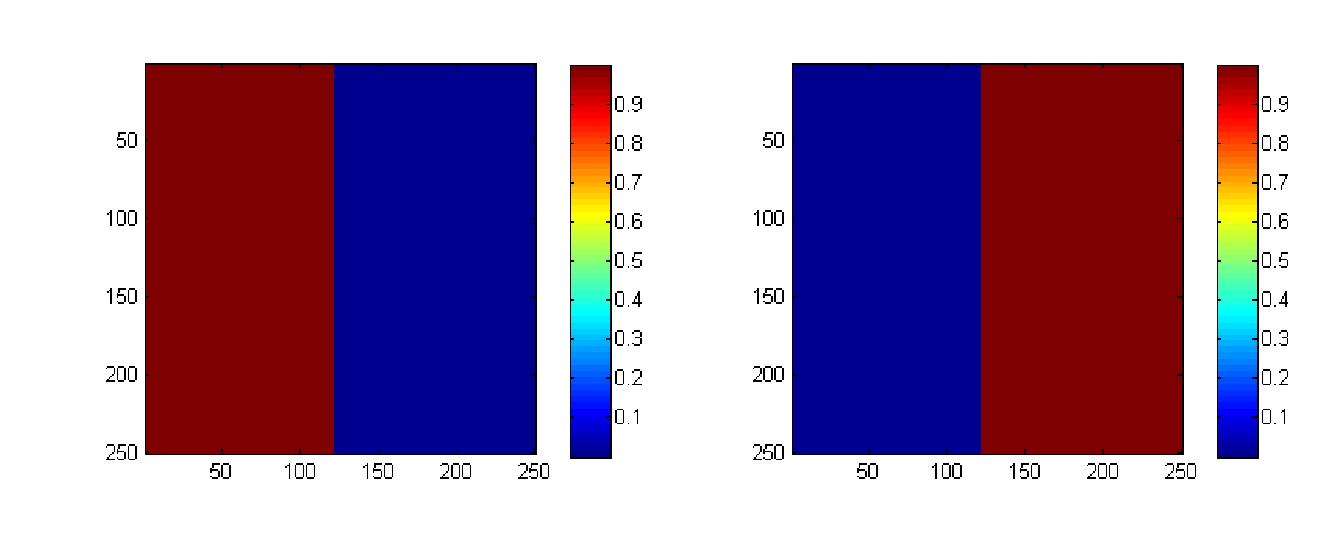
\includegraphics[scale=0.75]{images/mitad_mitad_clusters_sin_coordenadas_random}
\par\end{centering}

\caption{Clusterizacion con centroides aleatorios, sin coordenadas espaciales}
\end{figure}


\begin{figure}
\begin{centering}
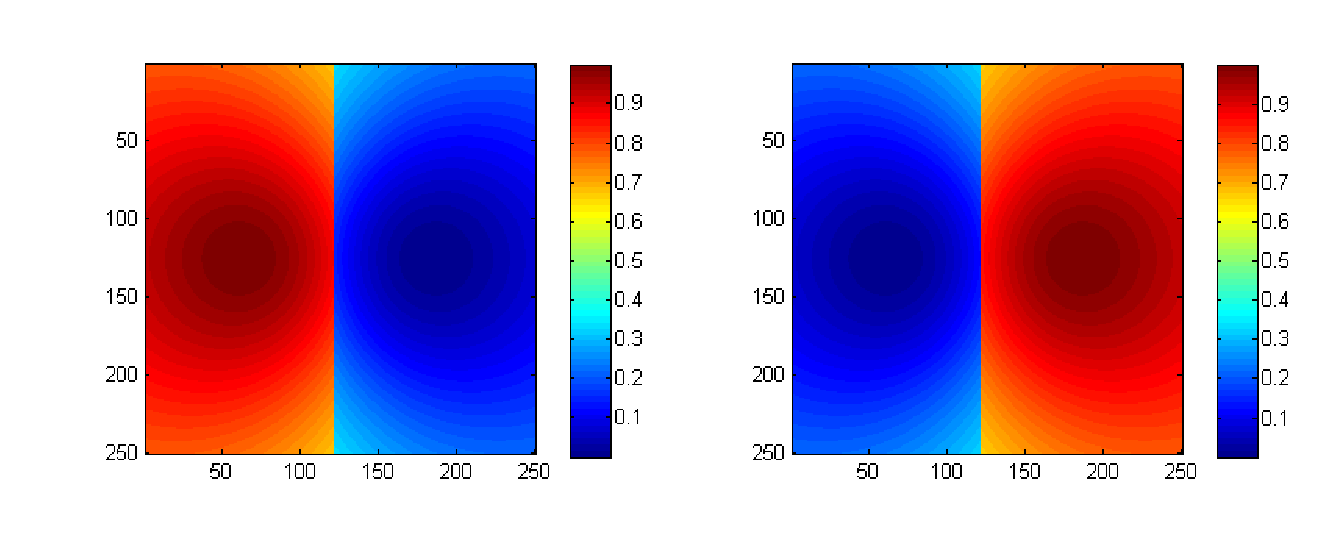
\includegraphics[scale=0.75]{images/mitad_mitad_clusters_con_coordenadas_random}
\par\end{centering}

\caption{Clusterizacion con centroides aleatorios y coordenadas espaciales}


\end{figure}


\begin{figure}
\begin{centering}
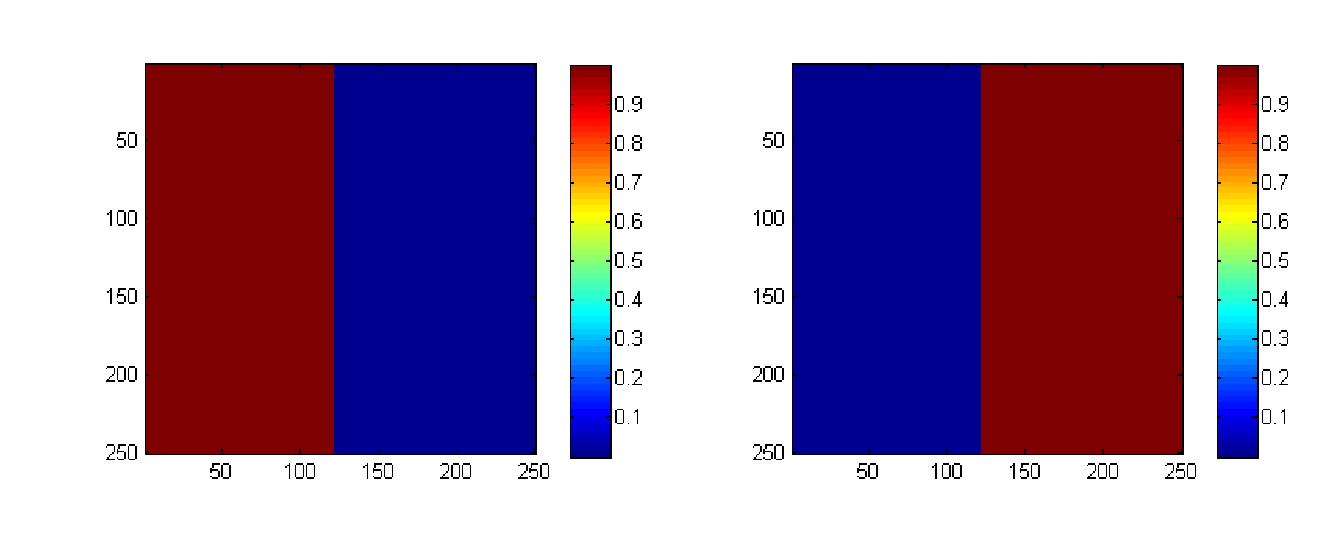
\includegraphics[scale=0.75]{images/mitad_mitad_clusters_sin_coordenadas_random}
\par\end{centering}

\caption{Clusterizacion con centroides iniciales seleccionados a mano sin coordenadas
espaciales}


\end{figure}


\begin{figure}
\begin{centering}
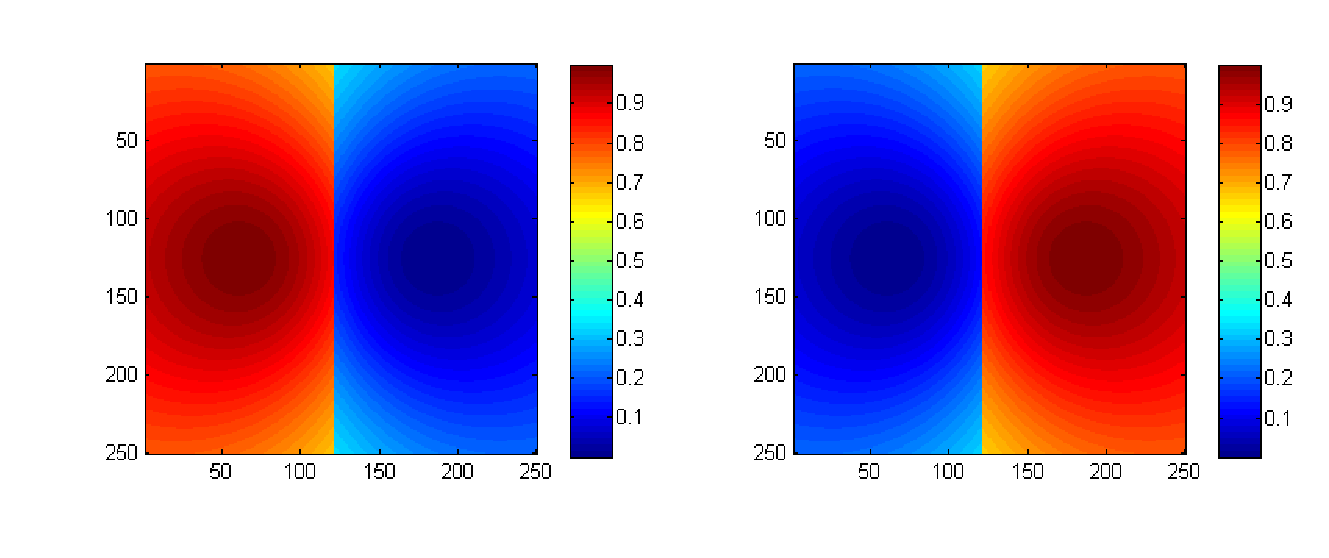
\includegraphics[scale=0.75]{images/mitad_mitad_clusters_con_coordenadas_centroide_manual}
\par\end{centering}

\caption{Clusterizacion con centroides iniciales seleccionados a mano y coordenadas
espaciales}


\end{figure}


\begin{figure}
\begin{centering}
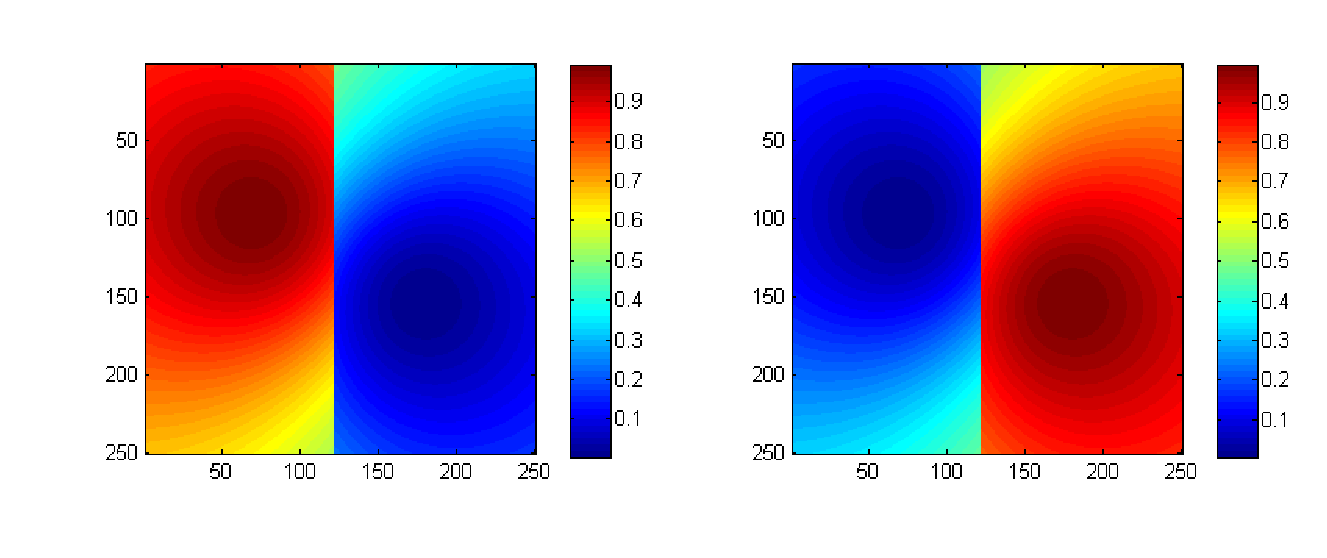
\includegraphics[scale=0.75]{images/mitad_mitad_clusters_con_coordenadas_centroide_manual_1iteracion}
\par\end{centering}

\caption{Clusterizacion con centroides iniciales seleccionados a mano, coordenadas
espaciales con una sola iteracion}


\end{figure}


\begin{center}
\begin{figure}
\begin{centering}
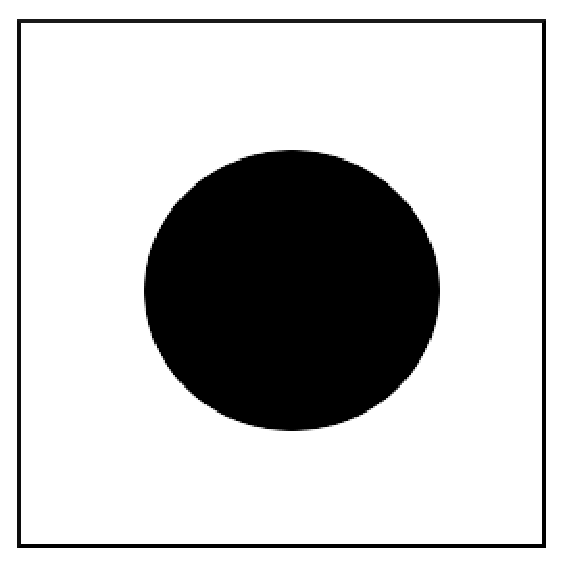
\includegraphics{images/circulo_250x250}
\par\end{centering}

\centering{}\caption{Imagen artificial zona cerrada}
\end{figure}

\par\end{center}
